% !TeX program = xelatex
\documentclass[
  convert={density=500, size=600, outext=.png}, 
  border=2pt
]{standalone}

\usepackage{fontspec}
\defaultfontfeatures{Ligatures={NoCommon,%
			NoDiscretionary,%
			NoHistoric,%
			NoRequired,%
			NoContextual}}
\setsansfont{Carlito}[%
	SmallCapsFeatures={Letters=SmallCaps},%
	SmallCapsFont={Roboto},%
	ItalicFeatures={SmallCapsFont=Roboto-Italic},%
	BoldFeatures={SmallCapsFont=Roboto-Bold},%
	BoldItalicFeatures={SmallCapsFont=Roboto-BoldItalic}%
]

\usepackage{tikz}
\usepackage{tikz-cd}
\usetikzlibrary{%
	calc,%
	arrows.meta,%
	arrows,%
	automata,%
	overlay-beamer-styles,%
	snakes,%
	shapes.arrows,%
	shapes.geometric,%
	shapes.symbols,%
	fit,%
	positioning,%
	decorations.pathreplacing,%
	backgrounds,%
}
\tikzset{
	>=Triangle,%
	nodes={align=center},%
	comp/.style={%
			draw,%
			rectangle,%
			very thick,%
			rounded corners,%
			minimum width=2.5cm,%
			minimum height=1cm,%
			fill=white},%
	input/.style={draw,%
			rectangle,%
			thick,%
			minimum width=2.5cm,%
			minimum height=1cm,%
			fill=white},%
	classnode/.style={%
			fill=cgreenlight,%
			rectangle,%
			draw,%
			inner xsep=0},%
	interfacenode/.style={%
			fill=corangelight,%
			rectangle,%
			draw,%
			inner xsep=0},%
	abstractclassnode/.style={%
			fill=cbluelight,%
			rectangle,%
			draw,%
			inner xsep=0},%
	inlinenode/.style={%
			inner xsep=.5cm,%
			minimum height=.6cm},%
}

\definecolor{reddy}{RGB}{172, 0, 51}
\definecolor{dkred}{rgb}{.6, 0, 0}
\definecolor{dkgreen}{rgb}{0, .5, 0}
\definecolor{dkblue}{rgb}{0, 0, .5}
\definecolor{cred}{RGB}{219, 68, 55}
\definecolor{credlight}{RGB}{250, 227, 225}
\definecolor{cgreen}{RGB}{3, 148, 77}
\definecolor{cgreenlight}{RGB}{209, 251, 230}
\definecolor{cblue}{RGB}{2, 119, 189}
\definecolor{cbluelight}{RGB}{208, 237, 254}
\definecolor{corange}{RGB}{173, 128, 2}
\definecolor{corangelight}{RGB}{253, 219, 123}
\newcommand{\cblue}[1]{\textcolor{cblue}{#1}}
\newcommand{\bfcblue}[1]{\textcolor{cblue}{\textbf{#1}}}
\newcommand{\cred}[1]{\textcolor{cred}{#1}}
\newcommand{\bfcred}[1]{\textcolor{cred}{\textbf{#1}}}
\newcommand{\cgreen}[1]{\textcolor{cgreen}{#1}}
\newcommand{\bfcgreen}[1]{\textcolor{cgreen}{\textbf{#1}}}
\newcommand{\corange}[1]{\textcolor{corange}{#1}}
\newcommand{\bfcorange}[1]{\textcolor{corange}{\textbf{#1}}}
\newcommand{\interfacename}[1]{\underline{\textbf{\textit{#1}}}}
\newcommand{\absclassname}[1]{\textbf{\textit{#1}}}
\newcommand{\classname}[1]{\textbf{#1}}

\usepackage{amsmath}
\usepackage{amsfonts}
\usepackage{amssymb}

\usepackage{silence}
\WarningsOff*


\begin{document}
\sffamily

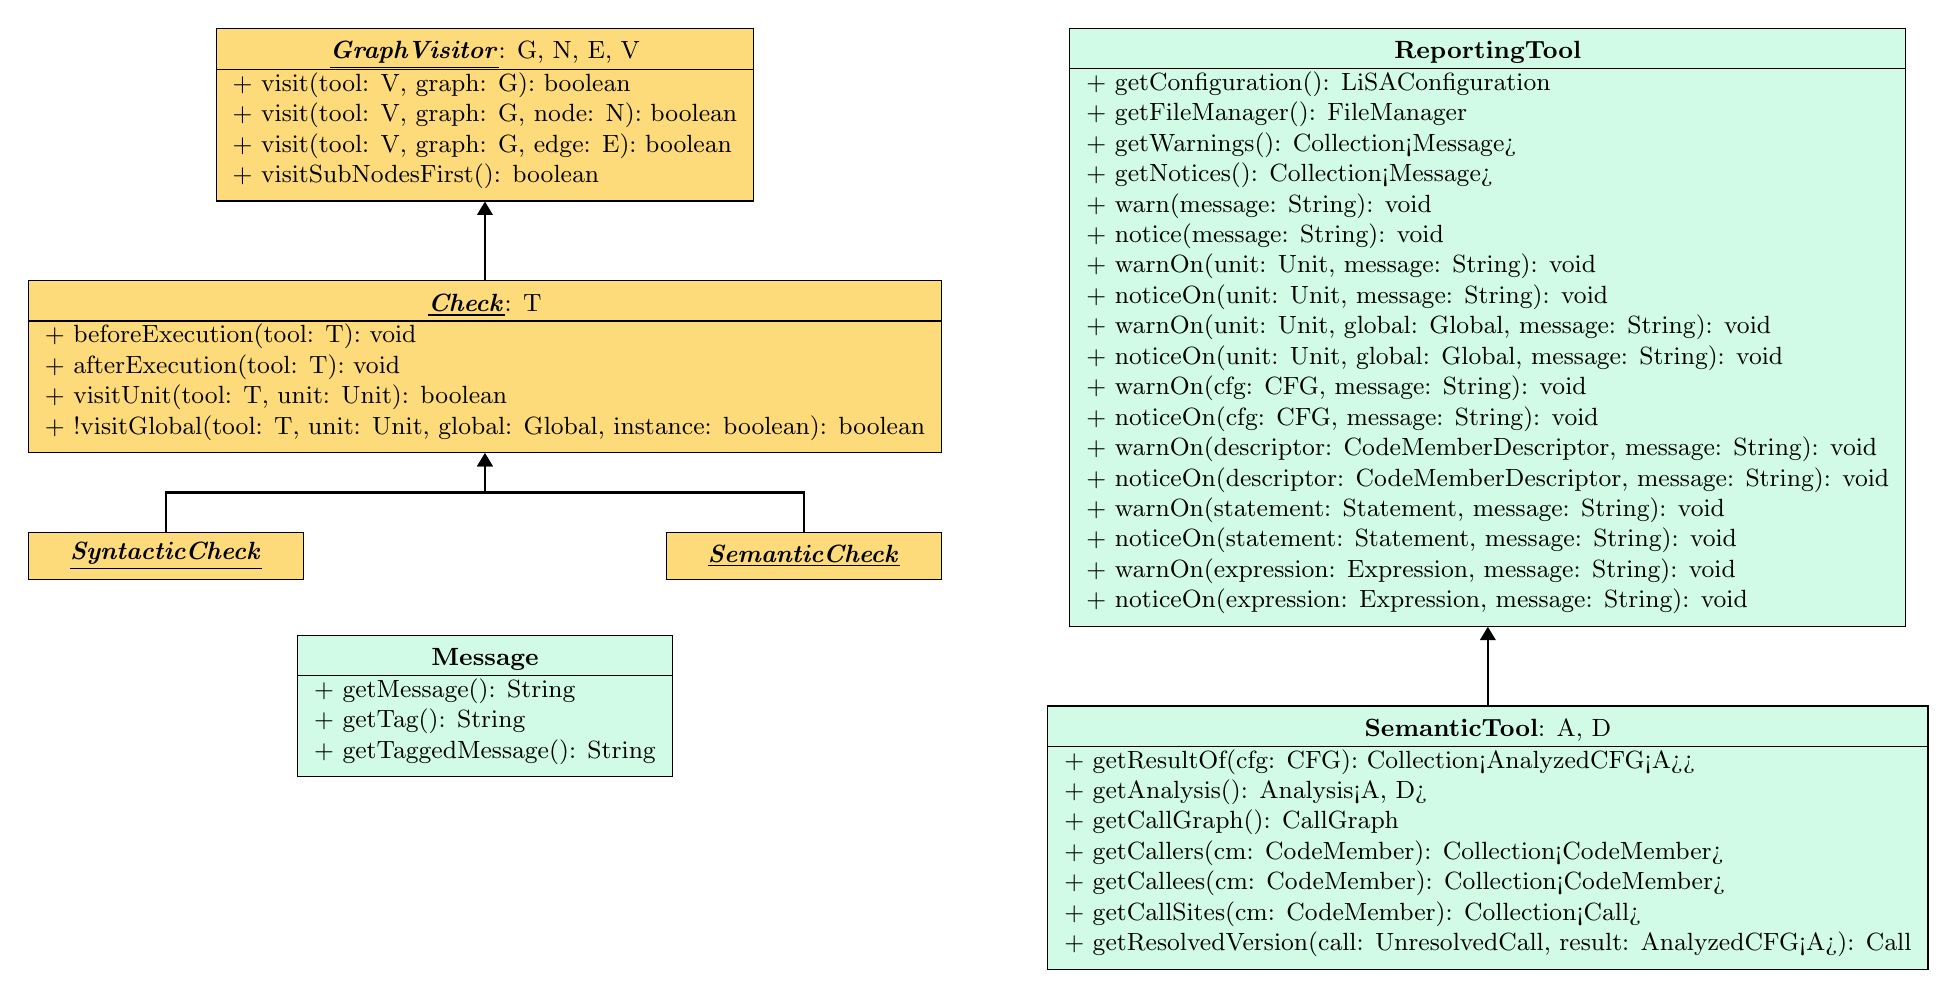
\begin{tikzpicture}[nodes={font={\small}, minimum width=3.5cm}]%
	\node[interfacenode] (visitor) {\begin{tabular}{l}
			\multicolumn{1}{c}{\interfacename{GraphVisitor}: G, N, E, V} \\
			\hline
			+ visit(tool: V, graph: G): boolean                          \\
			+ visit(tool: V, graph: G, node: N): boolean                 \\
			+ visit(tool: V, graph: G, edge: E): boolean                 \\
			+ visitSubNodesFirst(): boolean                              \\
		\end{tabular}};

	\node[interfacenode] (check) [below=of visitor] {\begin{tabular}{l}
			\multicolumn{1}{c}{\interfacename{Check}: T}                                    \\
			\hline
			+ beforeExecution(tool: T): void                                                \\
			+ afterExecution(tool: T): void                                                 \\
			+ visitUnit(tool: T, unit: Unit): boolean                                       \\
			+ !visitGlobal(tool: T, unit: Unit, global: Global, instance: boolean): boolean \\
		\end{tabular}};

	\node[interfacenode, inlinenode, below=of check.south west, anchor=north west] (syncheck) {\interfacename{SyntacticCheck}};
	\node[interfacenode, inlinenode, below=of check.south east, anchor=north east] (semcheck) {\interfacename{SemanticCheck}};

	\node[classnode] (msg) [below=of $(syncheck)!0.5!(semcheck)$] {\begin{tabular}{l}
			\multicolumn{1}{c}{\classname{Message}} \\
			\hline
			+ getMessage(): String                  \\
			+ getTag(): String                      \\
			+ getTaggedMessage(): String            \\
		\end{tabular}};

	\node[classnode, right=4cm of visitor.north east, anchor=north west] (reptool) {\begin{tabular}{l}
			\multicolumn{1}{c}{\classname{ReportingTool}}                       \\
			\hline
			+ getConfiguration(): LiSAConfiguration                             \\
			+ getFileManager(): FileManager                                     \\
			+ getWarnings(): Collection<Message>                                \\
			+ getNotices(): Collection<Message>                                 \\
			+ warn(message: String): void                                       \\
			+ notice(message: String): void                                     \\
			+ warnOn(unit: Unit, message: String): void                         \\
			+ noticeOn(unit: Unit, message: String): void                       \\
			+ warnOn(unit: Unit, global: Global, message: String): void         \\
			+ noticeOn(unit: Unit, global: Global, message: String): void       \\
			+ warnOn(cfg: CFG, message: String): void                           \\
			+ noticeOn(cfg: CFG, message: String): void                         \\
			+ warnOn(descriptor: CodeMemberDescriptor, message: String): void   \\
			+ noticeOn(descriptor: CodeMemberDescriptor, message: String): void \\
			+ warnOn(statement: Statement, message: String): void               \\
			+ noticeOn(statement: Statement, message: String): void             \\
			+ warnOn(expression: Expression, message: String): void             \\
			+ noticeOn(expression: Expression, message: String): void           \\
		\end{tabular}};

	\node[classnode, below=of reptool] (semtool) {\begin{tabular}{l}
			\multicolumn{1}{c}{\classname{SemanticTool}: A, D}                       \\
			\hline
			+ getResultOf(cfg: CFG): Collection<AnalyzedCFG<A>>                      \\
			+ getAnalysis(): Analysis<A, D>                                          \\
			+ getCallGraph(): CallGraph                                              \\
			+ getCallers(cm: CodeMember): Collection<CodeMember>                     \\
			+ getCallees(cm: CodeMember): Collection<CodeMember>                     \\
			+ getCallSites(cm: CodeMember): Collection<Call>                         \\
			+ getResolvedVersion(call: UnresolvedCall, result: AnalyzedCFG<A>): Call \\
		\end{tabular}};

	\draw[->, thick] (check) to (visitor);
	\draw[->, thick] (syncheck) |- ($(check.south)+(0,-0.5)$) to (check);
	\draw[->, thick] (semcheck) |- ($(check.south)+(0,-0.5)$) to (check);
	\draw[->, thick] (semtool) to (reptool);
\end{tikzpicture}

\end{document}
